% Build with latex, then convert the DVI with dvisvgm --no-fonts --exact.
% Arrow-shaped nodes encode DNA orientation. Links have no arrowheads.
% A node's head is its + side and its notched tail is its - side.
% Region (b) reverses the top node and all its incident sides. Its sequence
% is reverse-complemented (CT -> AG), preserving the represented walks.
\documentclass{article}
\usepackage[landscape,margin=1cm]{geometry}
\usepackage{lmodern}
\usepackage{tikz}
\usetikzlibrary{backgrounds,calc,decorations.pathreplacing}
\pgfdeclarelayer{paper}
\pgfdeclarelayer{links}
\pgfsetlayers{paper,background,links,main}
\pagestyle{empty}

% name, x, y, orientation, outline colour, fill colour, label
\newcommand{\seqnode}[7]{%
  \begin{scope}[shift={(#2,#3)},xscale=#4]
    \path[draw=#5,fill=#6]
      (-0.40,0.22) -- (0.24,0.22) -- (0.40,0) --
      (0.24,-0.22) -- (-0.40,-0.22) -- (-0.32,0) -- cycle;
    \coordinate (#1-center) at (0,0);
    \coordinate (#1-head) at (0.40,0);
    \coordinate (#1-tail) at (-0.32,0);
    \node[font=\large,inner sep=0pt] at (-0.04,0) {#7};
  \end{scope}%
}

\begin{document}
\noindent
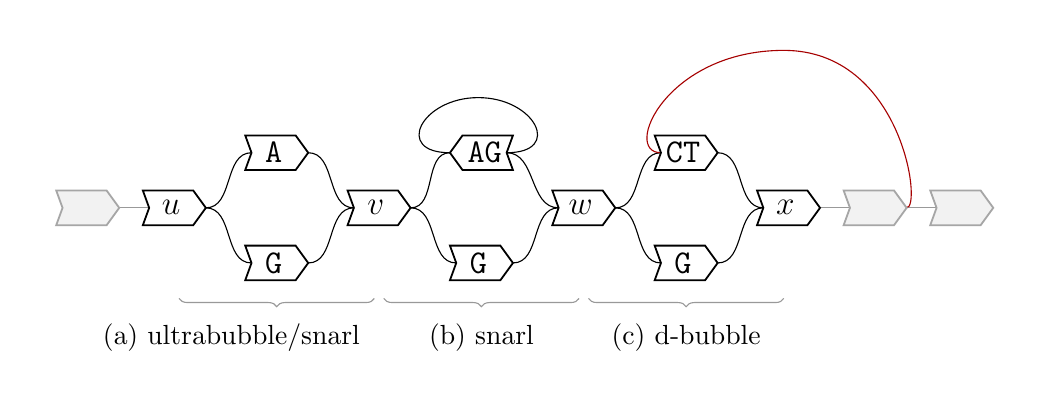
\begin{tikzpicture}[line width=0.65pt]
  \seqnode{s}{-1.1}{0}{1}{gray!70}{gray!10}{}
  \seqnode{u}{0}{0}{1}{black}{white}{$u$}
  \seqnode{a1}{1.3}{0.7}{1}{black}{white}{\texttt{A}}
  \seqnode{b1}{1.3}{-0.7}{1}{black}{white}{\texttt{G}}
  \seqnode{v}{2.6}{0}{1}{black}{white}{$v$}
  \seqnode{a2}{3.9}{0.7}{-1}{black}{white}{\texttt{AG}}
  \seqnode{b2}{3.9}{-0.7}{1}{black}{white}{\texttt{G}}
  \seqnode{w}{5.2}{0}{1}{black}{white}{$w$}
  \seqnode{a3}{6.5}{0.7}{1}{black}{white}{\texttt{CT}}
  \seqnode{b3}{6.5}{-0.7}{1}{black}{white}{\texttt{G}}
  \seqnode{x}{7.8}{0}{1}{black}{white}{$x$}
  \seqnode{c}{8.9}{0}{1}{gray!70}{gray!10}{}
  \seqnode{t}{10.0}{0}{1}{gray!70}{gray!10}{}

  \begin{pgfonlayer}{links}
    \draw[gray!80] (s-head) -- (u-tail);
    \foreach \nodeL/\nodeTop/\nodeBottom/\nodeR [count=\regionindex] in {
        u/a1/b1/v, v/a2/b2/w, w/a3/b3/x} {
      \ifnum\regionindex=2
        \draw (\nodeL-head) to[out=0,in=180] (\nodeTop-head);
        \draw (\nodeTop-tail) to[out=0,in=180] (\nodeR-tail);
      \else
        \draw (\nodeL-head) to[out=0,in=180] (\nodeTop-tail);
        \draw (\nodeTop-head) to[out=0,in=180] (\nodeR-tail);
      \fi
      \draw (\nodeL-head) to[out=0,in=180] (\nodeBottom-tail);
      \draw (\nodeBottom-head) to[out=0,in=180] (\nodeR-tail);
    }
    \draw[gray!80] (x-head) -- (c-tail);
    \draw[gray!80] (c-head) -- (t-tail);

    \coordinate (loop-top) at ($(a2-tail)!0.5!(a2-head)+(0,0.7)$);
    \draw (a2-tail)
      .. controls +(0.72,0) and +(0.72,0) .. (loop-top)
      .. controls +(-0.72,0) and +(-0.72,0) .. (a2-head);
    \coordinate (return-top) at ($(c-head)!0.5!(a3-tail)+(0,1.65)$);
    \draw[red!65!black] (c-head)
      .. controls +(0.20,0) and +(1.5,0) .. (return-top)
      .. controls +(-1.5,0) and +(-0.5,0) .. (a3-tail);
  \end{pgfonlayer}

  \foreach \labelnodeL/\labelnodeR/\regionletter/\regionkind [count=\annotationindex] in {
      u/v/a/{ultrabubble/snarl}, v/w/b/snarl, w/x/c/d-bubble} {
    \draw[gray!80,decorate,decoration={brace,mirror,amplitude=3pt}]
      ($(\labelnodeL-center)+(0.06,-1.15)$) --
      ($(\labelnodeR-center)+(-0.06,-1.15)$);
    \ifnum\annotationindex=1
      \node[font=\normalsize,anchor=east] at
        ($(\labelnodeR-center)+(-0.12,-1.65)$)
        {(\regionletter)\ \regionkind};
    \else
      \node[font=\normalsize] at
        ($(\labelnodeL-center)!0.5!(\labelnodeR-center)+(0,-1.65)$)
        {(\regionletter)\ \regionkind};
    \fi
  }
  \begin{pgfonlayer}{paper}
    \fill[white]
      ([xshift=-10pt,yshift=-8pt]current bounding box.south west) rectangle
      ([xshift=10pt,yshift=8pt]current bounding box.north east);
  \end{pgfonlayer}
\end{tikzpicture}
\end{document}
